\documentclass[UTF8,12pt,oneside]{ctexrep}

\usepackage[a4paper,top=2.5cm,bottom=2.5cm,left=2.7cm,right=2.7cm]{geometry}
\usepackage{booktabs}
\usepackage{longtable}
\usepackage{tabularx}
\usepackage{array}
\usepackage{enumitem}
\usepackage{setspace}
\usepackage{csquotes}
\usepackage{xurl}
\usepackage{graphicx}
\usepackage{float}
\usepackage[hidelinks]{hyperref}
\usepackage[backend=biber,style=numeric,sorting=none,maxbibnames=99]{biblatex}

\addbibresource{references.bib}

\setstretch{1.5}
\setlength{\parindent}{2em}
\setlength{\parskip}{0.35em}
\setlength{\emergencystretch}{2em}
\setlist[itemize]{leftmargin=2.2em,itemsep=0.2em,topsep=0.3em}
\setlist[enumerate]{leftmargin=2.2em,itemsep=0.2em,topsep=0.3em}
\newcommand{\Aegis}{\textbf{Aegis Runtime}}
\newcommand{\code}[1]{\texttt{#1}}
\graphicspath{{images/member3/}{../../docs/final-integration-assets/}}

\title{\bfseries Aegis Runtime：面向 AI Agent 的事务式安全执行架构\\[0.6em]
\large 作品报告}
\author{}
\date{}

\begin{document}

\maketitle
\tableofcontents

\chapter*{摘\quad 要}
\addcontentsline{toc}{chapter}{摘要}

大语言模型 Agent 已从文本生成扩展到文件读写、Shell 执行、网络访问和持久 Memory 等环境交互。相应地，安全问题不再局限于输入或输出内容，而必须覆盖真实副作用的产生、暂存、提交、取消与恢复。\Aegis{} 面向这一需求实现了事务式安全执行 Runtime：所有工具调用经过风险分类、策略与权限判定、受控执行、检查、提交或回滚，并将全过程记录为可追溯的 Audit 事件。

本作品的三项核心创新为：（1）\textbf{Transactional Controlled Execution}：将可恢复副作用置于 Pending 状态，并以 Checkpoint、Commit Gate 和 Effect 生命周期约束可信状态的形成；（2）\textbf{Approval-aware TaskGraph Scheduling}：在任务图中仅阻断等待审批节点的依赖或资源冲突范围，使安全独立节点能够继续推进；（3）\textbf{Dependency-aware Selective Rollback}：回滚受影响依赖闭包内的 Effect，保留未进入受影响范围且已安全提交的独立 Effect。Risk、Policy、Permission、Approval 与 Audit 是上述运行时链路的支撑机制，而非对核心创新的替代命名。

最终验收覆盖静态检查、后端、前端和真实浏览器流程：Ruff 通过，Pyright 为 0 errors、0 warnings；后端测试为 889 passed、8 skipped；前端 Vitest 为 14 passed；Playwright 为 11 passed。正式实验数据固定为 Safety 225 行、Graph 18 行和 Rollback 105 行，并由原始数据及聚合结果重建核验。Safety 使用确定性受控规则，不以 LLM 裁决作为正式结论依据；Graph 在固定时延、确定性受控环境中验证工程行为，不作统计显著性主张。

\vspace{1em}
\noindent\textbf{关键词：} Agent 安全；事务式受控执行；审批感知调度；选择性回滚；状态完整性

\chapter{作品概述}

\section{作品背景}

Agent 将语言模型的决策接入外部工具后，系统可能读取不可信文档、修改文件、执行命令或形成跨任务的持久状态。间接提示注入已经表明，第三方内容可能被模型错误解释为高优先级指令，从而诱导集成应用执行非预期操作\cite{greshake2023indirect}。代码 Agent 的风险评测也将危险命令和执行环境置于问题中心\cite{guo2024redcode}。因此，安全 Runtime 必须把控制点放在副作用发生的位置，而不是仅依赖对输入、输出或模型意图的单点判断。

\section{问题定义与威胁模型}

本作品处理的对象是携带工具调用请求和任务契约的 Agent 运行时。对于每一项动作，系统需要判断它是否符合用户目标与授权边界、是否允许在安全结论确定前进入隔离状态，以及失败或取消时应恢复哪些状态。为此，系统从以下四个层面描述威胁模型：

\begin{itemize}
  \item \textbf{指令层：}网页、文档与工具输出中的不可信内容可能携带间接提示注入或语义操纵；
  \item \textbf{资源层：}路径越界、危险 Shell、敏感文件访问与未授权外发可能直接产生高风险副作用；
  \item \textbf{状态层：}未经验证的工具结果或 Memory 写入若直接成为可信状态，可能造成跨任务持续污染\cite{dash2026memorypoisoning}；
  \item \textbf{调度层：}审批等待、取消与恢复若未正确约束，可能造成兄弟节点泄漏、孤儿执行或重复执行\cite{khan2026stop}。
\end{itemize}

系统将 Planner 输出视为不可信提案。可信边界由 Runtime Scheduler、风险策略与权限判定、审批门、Effect 生命周期和 Audit 记录共同构成；工具原始输出不直接成为可信 Memory，也不以原始不可信内容展示给前端。

\section{国内外研究现状}

研究界已从风险发现逐步走向 Agent 运行时治理。ToolEmu 通过模拟工具环境识别工具使用中的长尾风险\cite{ruan2024toolemu}；R-Judge 与 Agent Security Bench（ASB）分别聚焦交互轨迹风险意识和多场景攻防评测\cite{yuan2024rjudge,zhang2025asb}；AgentHarm 则从多步恶意任务角度评估 Agent 被滥用的风险\cite{andriushchenko2025agentharm}。这些工作表明，安全评估需要覆盖多步轨迹和真实工具影响，而不能只观察文本拒答。

在运行时防护方面，SafeAgent 将安全建模为随轨迹演化的有状态决策问题\cite{liu2026safeagent}；SafeHarness 将控制机制置于 Agent 生命周期和执行 Harness 中\cite{lin2026safeharness}；Consent Integrity 强调审批内容必须由可信中介绑定到实际执行对象\cite{weng2026consent}。Cordon 已将工具意图、结果血缘、暂存 Effect 与审计元数据置于任务级语义事务之中\cite{chen2026cordon}。这些工作说明，\Aegis{} 不将“事务”或“审批”本身宣称为首创，而将重点放在三项机制在可运行 Runtime 中的受控组合、工程闭环与可复现验证。

\section{设计目标}

\Aegis{} 的设计目标是使安全判断、任务推进和状态恢复处于同一条可验证链路中。首先，所有真实副作用经由统一 Runtime Scheduler 进入受控执行，风险未确定或权限不足时采用 Fail-Closed 行为。其次，可恢复的文件、下载与 Memory 状态遵循 Pending 到可信状态的生命周期；检查失败、拒绝或取消时，系统据已冻结的关联关系恢复受影响范围。再次，审批不成为全局暂停信号：仅依赖等待节点或与其 Effect target 冲突的节点被阻断，无依赖且无冲突的节点可继续调度。最后，Risk、Policy、Permission、Approval、Checkpoint、Effect、Commit/Rollback 和 Audit 都形成结构化事实，以支持全过程审计可追溯性。

\section{适用范围与边界}

\Aegis{} 适用于需要工具调用、运行时审计、人工审批和受控恢复的本地或企业自动化工作流，例如安全敏感代码辅助、文件处理和多步骤业务准备流程。当前原型未覆盖分布式调度、服务重启恢复、完整 ACID 事务、真实支付或邮件发送、通用 MCP/Skill 协议，以及同一节点 speculative execution。对外发类动作，系统以受控、脱敏和干运行边界为前提；本作品不据此声称对开放网络环境中的任意副作用完成通用回滚。

\chapter{作品设计与实现}

\section{统一运行时链路}

\Aegis{} 将 Planner 输出视为不可信提案，并在工具调用进入真实资源之前统一经过风险分类、Policy 与 Permission 判定、必要的 Approval、受控执行以及 Audit 记录。Risk、Policy、Permission、Approval 和 Audit 在这里承担的是运行时支撑职责：它们把请求、决策、状态转换和资源关联形成可检索的脱敏事实，并不替代本作品的三项核心创新。

任务由带依赖边的 TaskGraph 表示。高风险节点进入 \code{WAITING\_APPROVAL} 时，系统只约束该节点的后继或同一 Effect target 的冲突范围；无依赖且无冲突的节点仍可继续。Grant 后受影响图恢复推进，Deny 或 Cancel 后相关节点收敛。当前原型明确不支持同一节点的 speculative overlap（\code{NOT\_SUPPORTED}），也未覆盖分布式调度或服务重启恢复。

\section{Transactional Controlled Execution}

对文件、Memory 和下载等可恢复副作用，运行时采用 Checkpoint、Pending Effect、验证、Commit、Rollback 与 Cleanup 的受控链路。候选结果先登记为 \code{PENDING}，并携带 task、request、规范化 target、Checkpoint 与摘要关联；只有必要校验通过后才转为 \code{COMMITTED}。取消、拒绝或验证失败时，执行器依据已登记的关联关系恢复可逆资源，并将对应事实标记为 \code{ROLLED\_BACK}、\code{REJECTED} 或 \code{CLEANED}。图~\ref{fig:effect-lifecycle} 给出统一生命周期。

\begin{figure}[H]
  \centering
  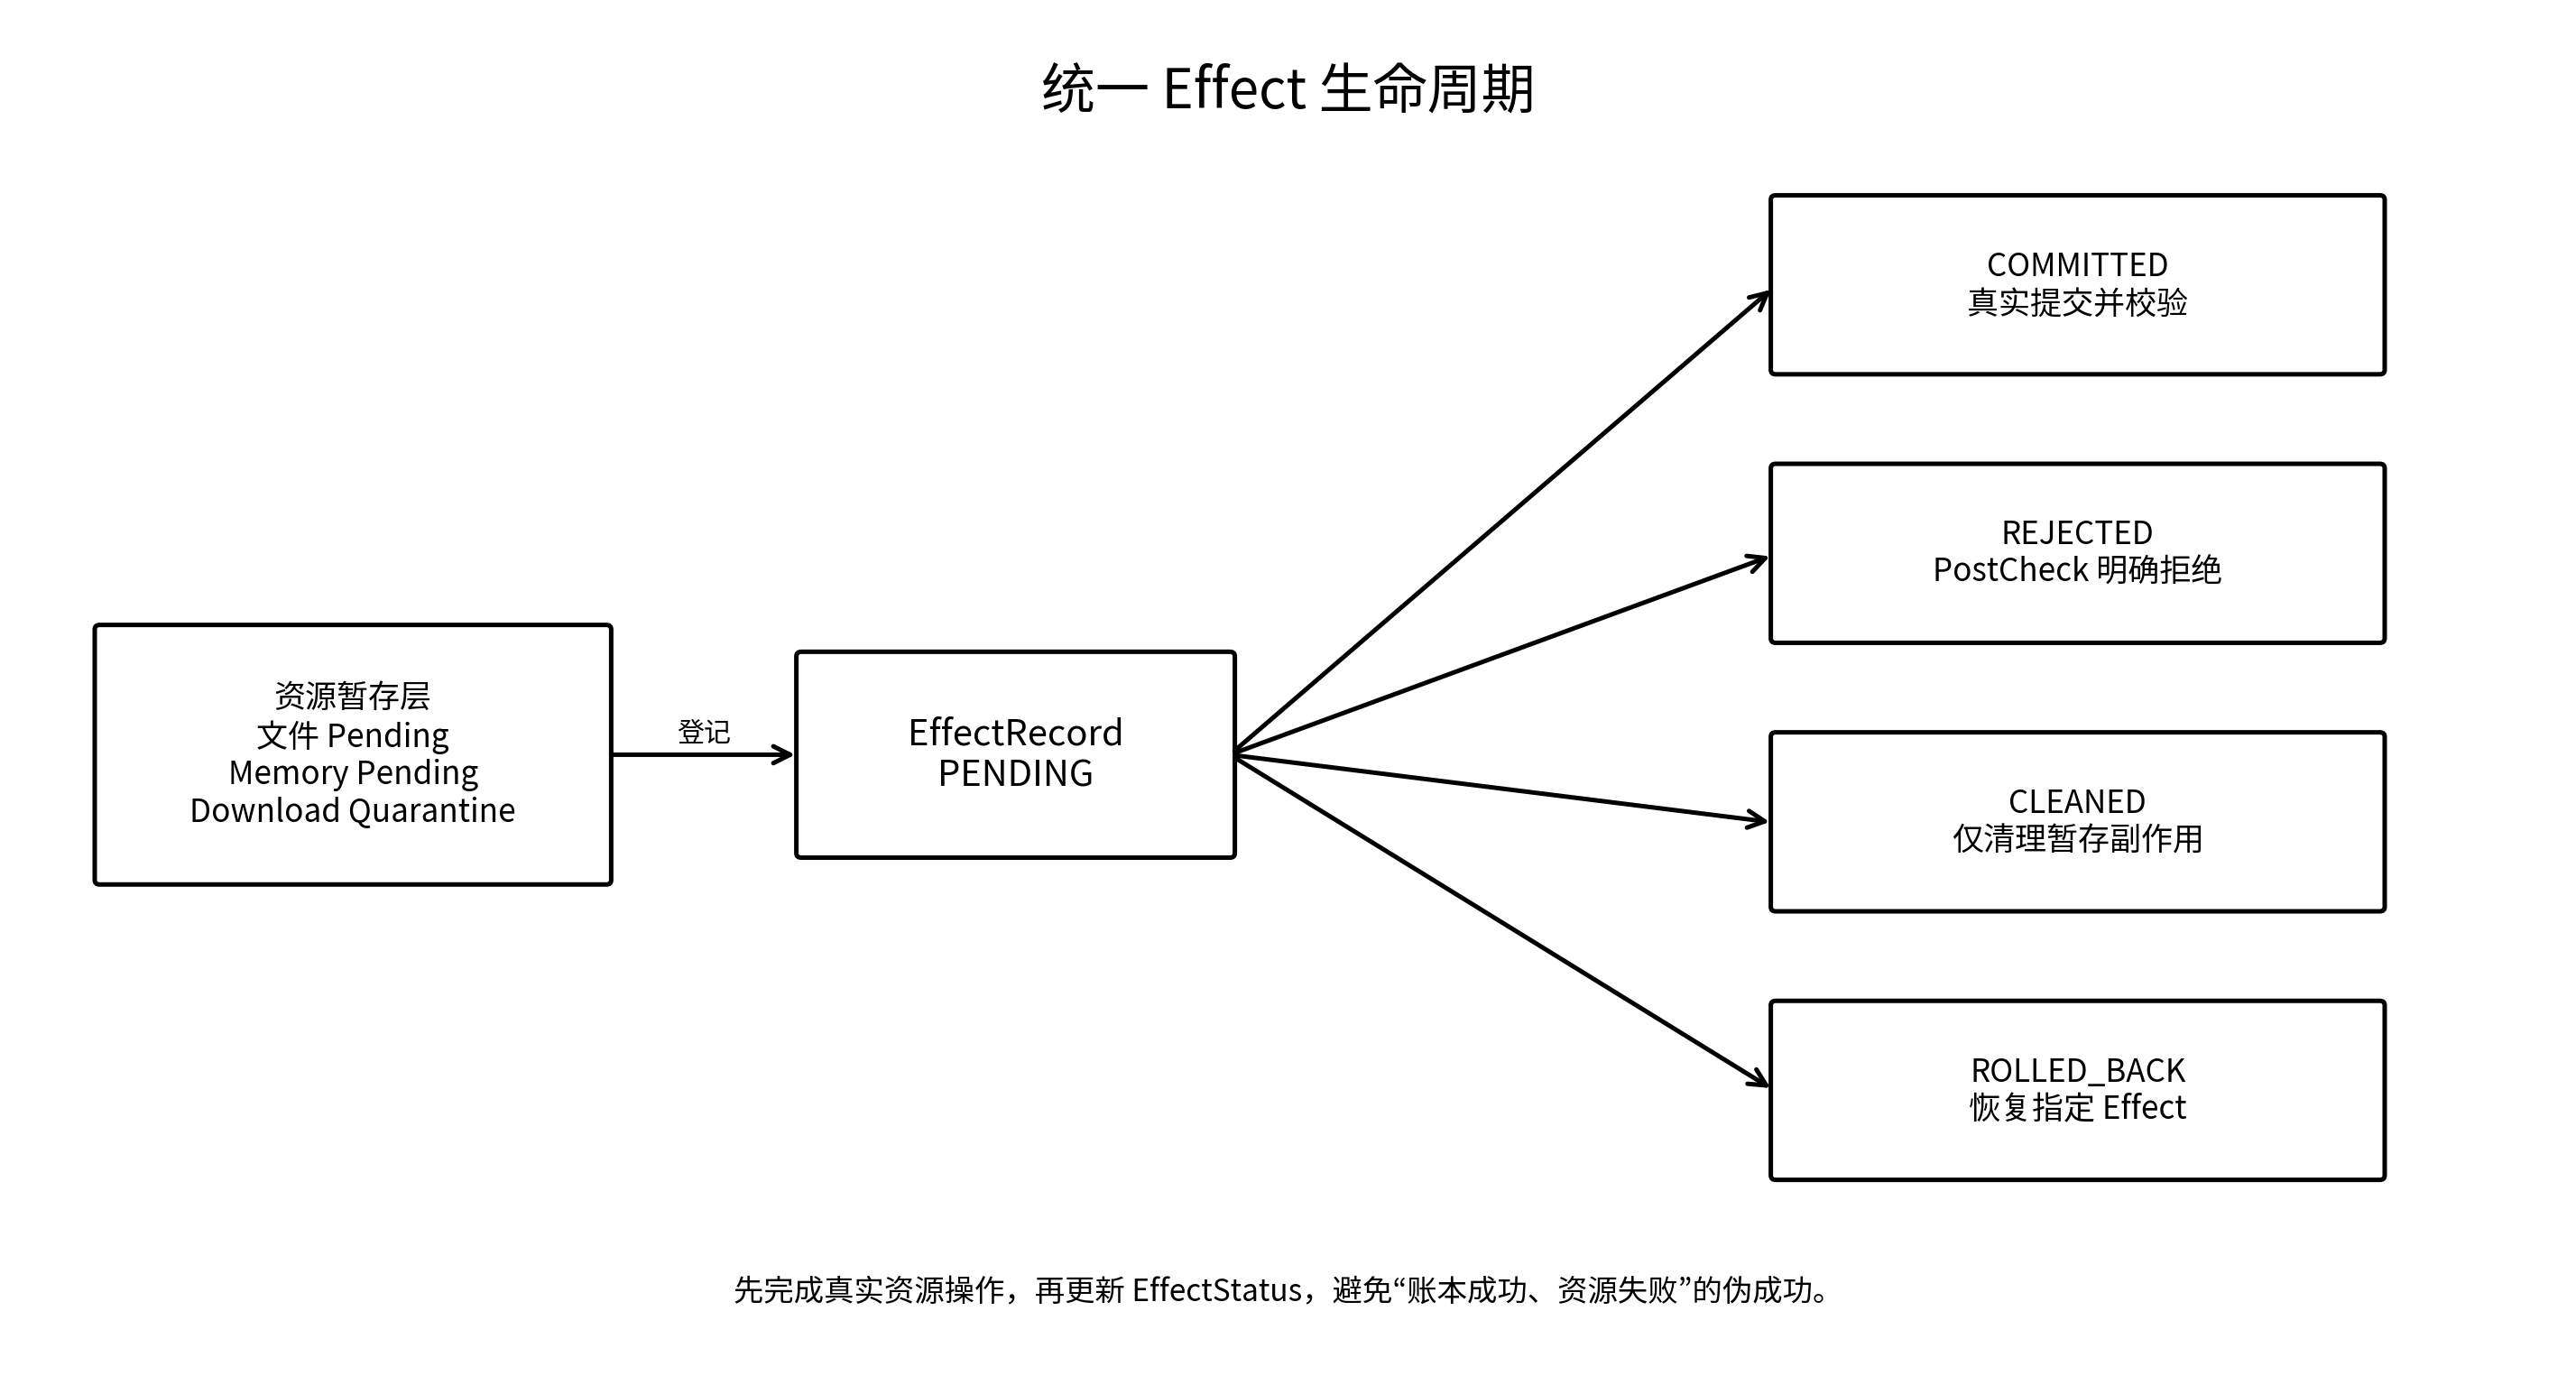
\includegraphics[width=0.94\linewidth]{effect_lifecycle.png}
  \caption{受控副作用的 Effect 生命周期}
  \label{fig:effect-lifecycle}
\end{figure}

这种“事务式”表述限定为工程级的受控提交与恢复语义：它不宣称完整 ACID、分布式事务或对不可逆外部世界副作用的通用撤销。前端只展示 Effect kind、脱敏 target reference、Checkpoint 标识、状态以及回滚或保留原因；不展示密钥、原始不可信工具输出或隐藏推理。

\section{Memory 状态完整性与审批感知调度}

Memory 写入以可信状态为边界：新记录在通过校验前不进入可信检索；批准提交后才成为可用状态。撤销某个新版本时，运行时仅恢复该 Key 的先前可信版本，其他 Key 与独立版本不进入撤销范围。结合 TaskGraph，审批、取消与恢复都以 task、node、request、Effect 和 Checkpoint 的关联关系为依据；浏览器端的 Approval、Graph、Effect、Audit 与 Dashboard 使用同一 task 标识查询，并以脱敏投影展示状态。

\section{Dependency-aware Selective Rollback}

选择性回滚通过显式范围与依赖关系决定处理集合。执行前的 Preflight 校验 Effect、request、Checkpoint 和 task 的归属；跨任务引用、未知对象或关联不一致的计划会在产生资源变化前被拒绝。执行时，系统回滚受影响依赖闭包内的 Effect，并保留未进入该范围且已安全提交的独立 Effect。图~\ref{fig:selective-rollback} 描述了目标 Effect 被回滚、独立 Effect 被保留的机制。

\begin{figure}[H]
  \centering
  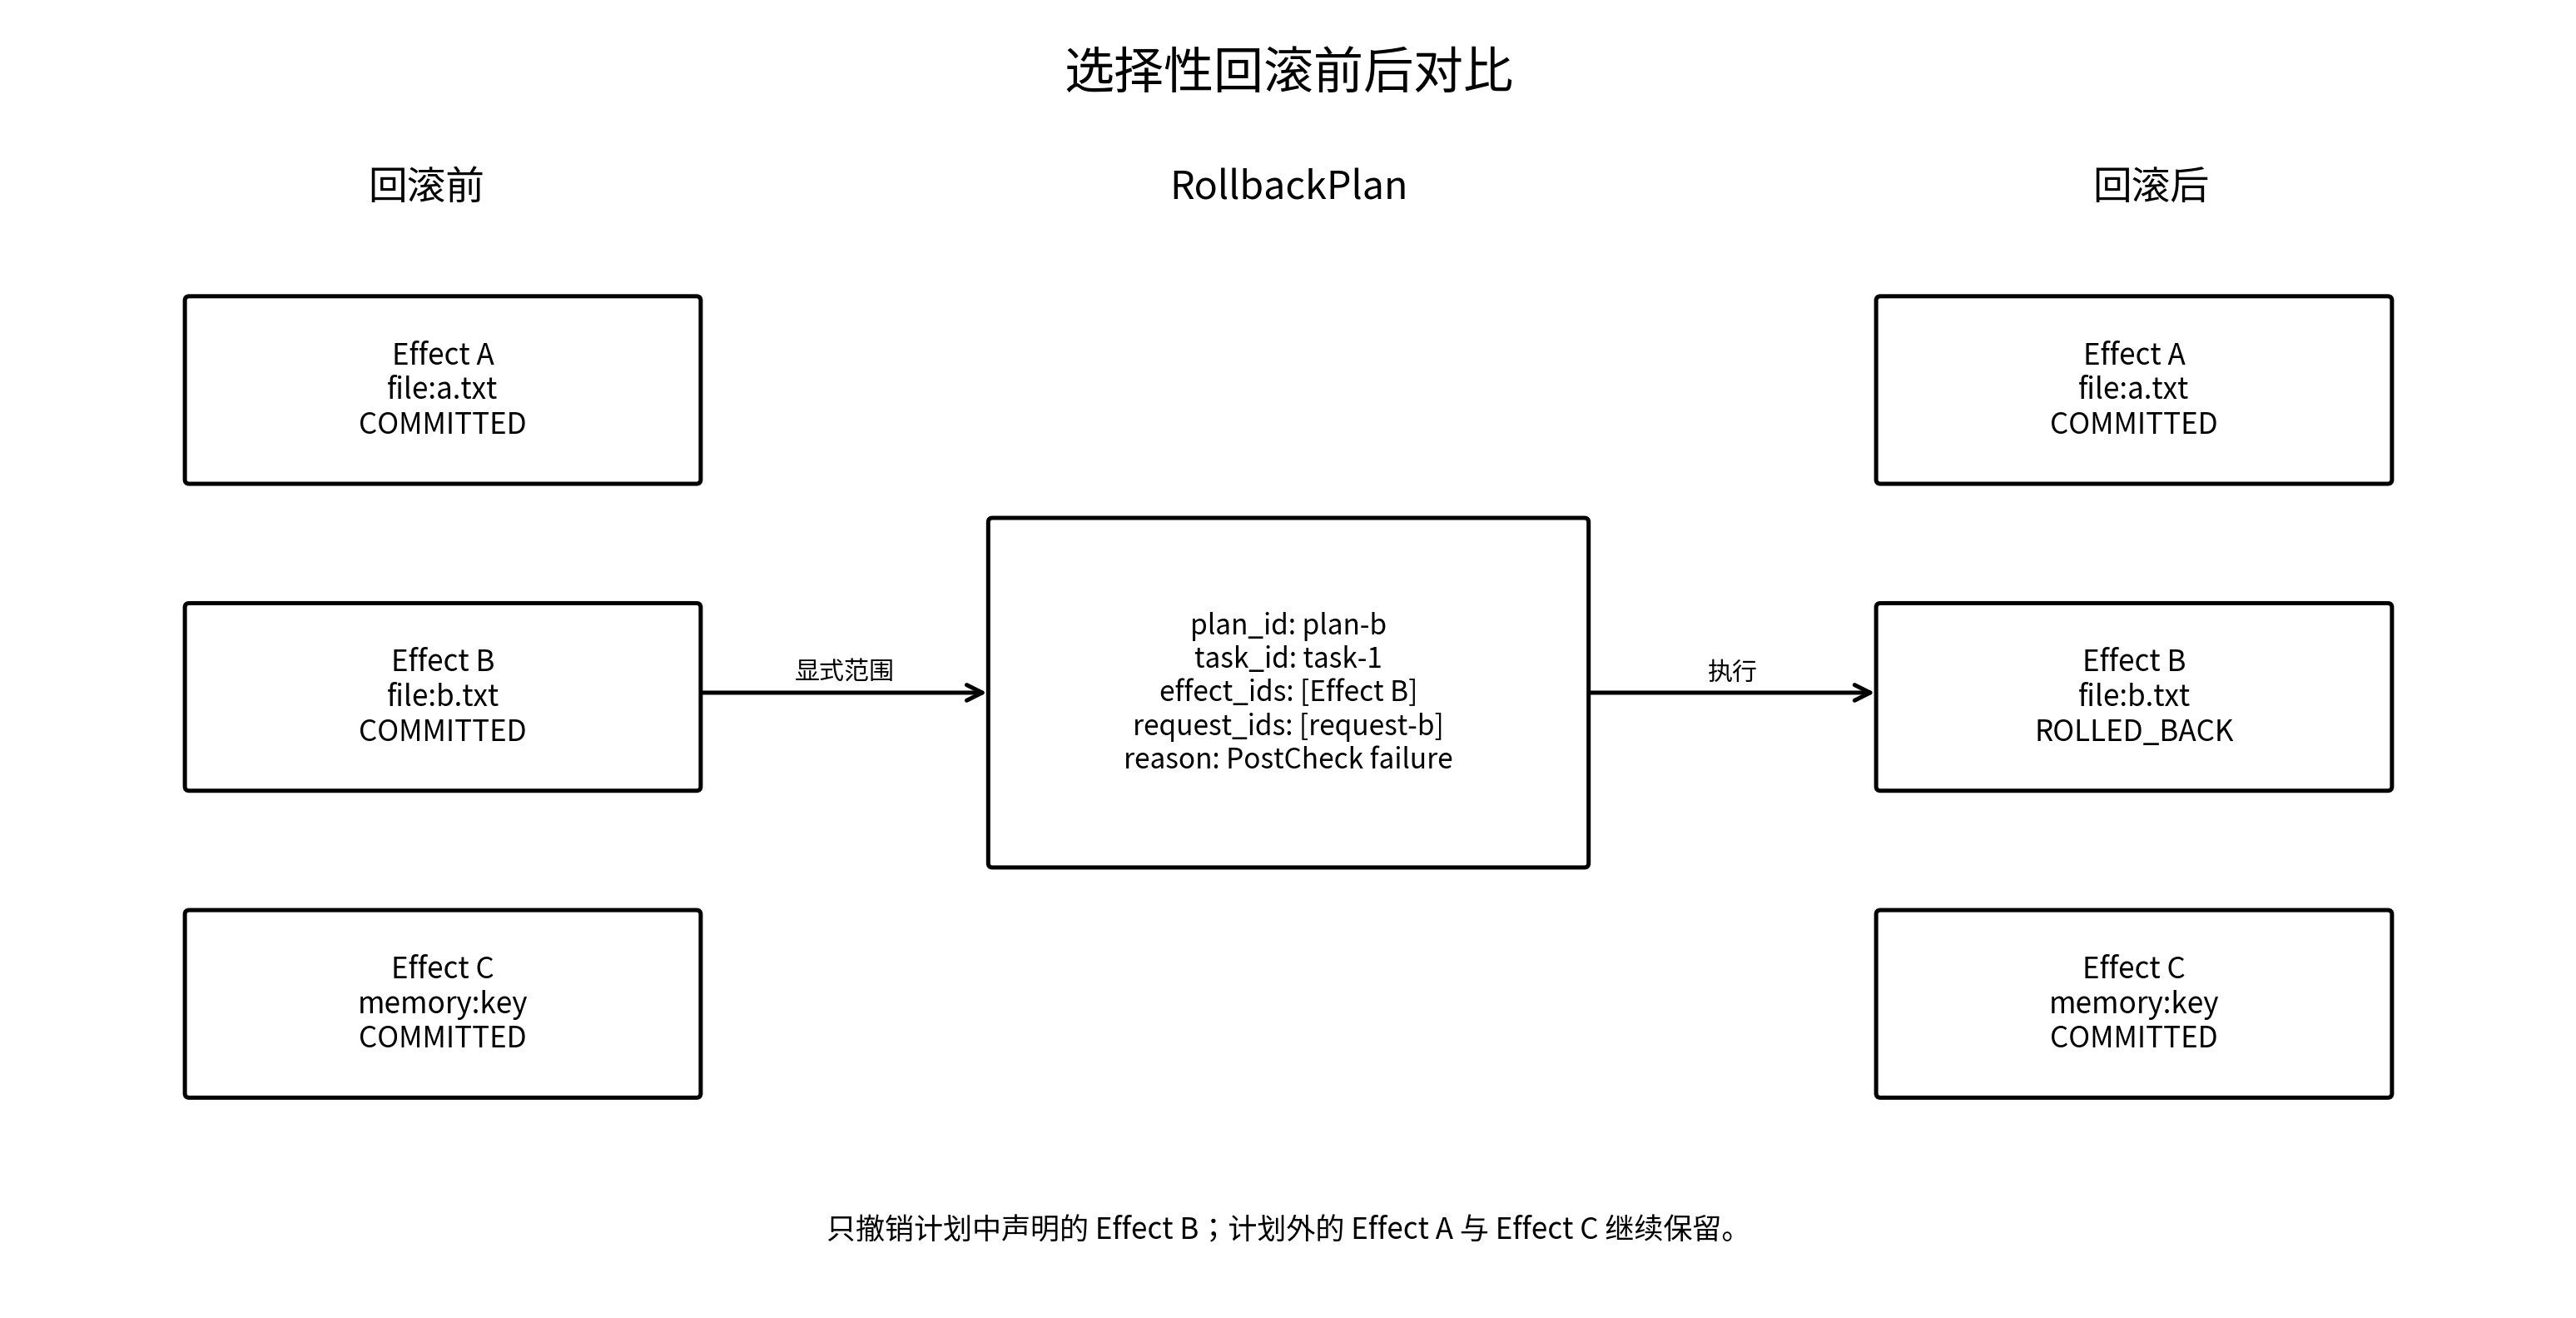
\includegraphics[width=0.94\linewidth]{selective_rollback_before_after.png}
  \caption{依赖感知选择性回滚与独立 Effect 保留}
  \label{fig:selective-rollback}
\end{figure}

资源目标以规范化 \code{target\_ref} 关联，同一目标按既定关联顺序恢复，计划外目标不进入回滚队列。若提交后检测到用户再次修改，系统保留用户内容并记录残留与原因，不以旧 Checkpoint 覆盖新内容。重复执行同一已完成计划不会重复修改资源；Cancel 后 Resume 返回冲突状态，从而避免终态任务被重新启动。

\chapter{作品测试与分析}

\section{测试思路与评价原则}

本作品的测试不把“能否运行一次”作为唯一标准，而是关注安全机制在完整任务过程中的行为是否符合预期。Agent 运行时涉及风险判断、人工审批、任务图推进、资源提交和状态恢复等多个环节，如果只检查某一个函数是否返回成功，无法说明这些环节在取消、拒绝或异常情况下是否仍能保持一致。因此，测试设计围绕三个问题展开：危险或越权动作能否在执行边界被识别和处置；审批等待时任务图能否既保持安全边界又允许独立工作继续；当任务取消或局部失败时，系统能否恢复受影响状态并保留独立成果。

为使结果可复核，三组正式实验均使用固定的 fixtures、明确的预期结果和重复运行记录。Safety 实验关注风险、策略、审批与审计；Graph 实验关注依赖关系、审批等待和节点推进；Rollback 实验关注 Effect 范围、状态恢复和独立成果保留。每一组实验都不通过人工填写结果，而是根据运行记录自动汇总；对同一场景的多次运行可以检查重复次数、场景覆盖和结果的一致性。表~\ref{tab:formal-data} 概括三组实验的规模和验证对象。

\begin{table}[H]
  \centering
  \caption{三组正式实验的规模与验证对象}
  \label{tab:formal-data}
  \begin{tabularx}{\linewidth}{l c c X}
    \toprule
    实验组 & 记录数量 & 实验设置 & 主要验证内容 \\
    \midrule
    Safety & 225 条 & 15 个安全场景、3 种模式、每种 5 次重复 & 风险升级、策略阻断、审批与审计事实 \\
    Graph & 18 条 & 2 个图调度场景、3 种模式、每种 3 次重复 & 审批等待与独立节点推进的调度行为 \\
    Rollback & 105 条 & 7 个回滚场景、3 种模式、每种 5 次重复 & Effect 范围、恢复结果与独立成果保留 \\
    \bottomrule
  \end{tabularx}
\end{table}

这些实验服务于工程行为验证，而不是将小样本、固定环境下的结果解释为开放环境中的统计结论。特别是 Graph 实验采用固定时延和确定性受控环境，其意义在于验证审批状态与依赖关系是否按照设计发生变化，而不是比较真实大模型在不同时段的性能波动。

\section{Safety 实验：验证风险处置是否到达执行边界}

Safety 实验的背景是：Agent 面对的危险并不只是一条明显的恶意命令。提示注入可能把外部文本伪装成任务指令，路径访问可能越出允许范围，危险 Shell 可能破坏本地环境，未经许可的外发可能泄露敏感信息，未经核验的 Memory 写入则可能影响后续任务。因此，安全机制需要在工具真正执行之前完成风险识别与处置，而不是在造成影响后仅给出文字解释。

实验设置覆盖十五个固定场景，包括危险 Shell、路径越界、回环下载、未授权外发、Memory 污染、提示注入、需要审批的敏感读取、拒绝删除、正常读取和正常写入等。每个场景都给出预期状态，例如高风险动作应当被阻断或进入审批，正常动作在满足规则后可以继续。三种模式用于比较没有完整运行时约束、采用完整保护以及采用自适应运行时策略时的行为差异；每种模式对每个场景重复五次，形成 225 条正式记录。

选择这些场景的原因在于它们分别对应不同的风险入口。危险 Shell 和路径越界检验本地资源边界；下载和外发检验网络边界；提示注入和 Memory 污染检验不可信信息能否改变后续行为；审批场景检验用户决定是否真正绑定到目标操作；正常场景则检验安全机制不会把所有操作一律拒绝。这样，实验既关注“危险动作是否被拦住”，也关注“安全动作是否能在授权条件下继续”。

实验结果以每个场景的状态匹配、风险升级、审批事实、人工动作和工具执行事实进行核验。完整保护和自适应运行时模式将风险判断、策略处置与审计记录放在同一链路中：需要审批的动作不会绕过等待状态，明确禁止的动作不会进入真实执行，安全动作则在满足条件后继续。对照模式的意义在于显示缺少相应运行时约束时会出现的差异，而不是把它与最终安全机制混为一谈。由于整个实验使用确定性规则和固定 fixtures，正式结论不依赖 LLM 对同一输入作出的偶然判断。

Safety 实验说明，风险识别只有与执行边界、审批和审计记录连接起来，才能转化为可验证的安全行为。单独给出“风险较高”的提示并不能阻止工具继续调用；只有当系统能够改变节点状态、阻断请求或要求明确授权时，风险策略才真正参与了运行时控制。

\section{Graph 实验：验证审批等待中的任务推进}

Graph 实验关注一个常见矛盾：高风险节点需要等待用户审批，但整个任务不应因此无条件冻结。若系统只暂停高风险节点，却允许其依赖节点或资源冲突节点继续执行，审批就可能失去实际意义；若系统暂停全部节点，又会让原本安全、独立的工作无谓停滞。Approval-aware TaskGraph Scheduling 的目标是在两者之间建立清晰边界。

实验设置包含“审批等待”和“并行依赖图”两个固定场景。在审批等待场景中，一个节点需要人工确认，另一个独立节点不依赖该动作；在并行依赖图场景中，节点之间存在明确的先后关系和可并行部分。每个场景在三种模式下重复三次，共形成 18 条正式记录。记录关注图完成时间、审批等待时间、等待期间完成的独立节点数量以及是否产生额外的并行节省时间等指标。

设置审批等待场景，是为了检查等待状态是否真正成为边界：目标节点在获得 Grant 前不能继续，依赖它的后续节点不能跨越该边界；与此同时，与其无依赖且无资源冲突的节点可以按照规则完成。设置并行依赖图场景，则是为了检查系统是否能够正确区分“可以独立推进”和“必须等待前置条件”的节点，而不是单纯按提交顺序串行执行全部任务。

实验记录表明，在采用审批感知调度的模式下，等待审批的节点会保持在相应状态，独立节点能够按规则推进；Grant 后图继续收敛，Deny 或 Cancel 后受影响路径停止并进入终态。固定时延环境使这些结果主要反映状态机与调度逻辑，而非网络或模型响应的随机波动。由此可以说明，审批不只是一个额外弹窗，而是能够参与图调度决策的运行时状态。

Graph 实验同样明确了作品的边界：当前系统不支持同一节点内部的 speculative overlap，也不把这组固定环境下的重复运行解释为对大规模分布式调度能力的证明。实验验证的是“审批边界、依赖关系和独立推进能否保持一致”这一工程问题。

\section{Rollback 实验：验证局部恢复与独立成果保留}

Rollback 实验针对的背景是，Agent 任务往往包含多项资源操作。任务被取消、提交异常或用户发现结果不合适时，若系统只能把整个任务全部清空，就会误伤已经安全完成的独立成果；若系统什么都不恢复，又可能留下不应继续存在的文件、Memory 或下载对象。选择性回滚需要解决的正是“恢复到什么范围”为止的问题。

实验包含七个 Case：文件选择性回滚、Memory 版本恢复、提交失败、用户修改冲突、幂等重试、跨任务范围拒绝和下载隔离回滚。文件场景检查系统能否只恢复目标文件；Memory 场景检查新版本撤销后此前可信版本能否重新可见；提交失败场景检查受控状态能否在失败后处理；用户修改冲突场景检查系统是否避免用旧 Checkpoint 覆盖用户后来写入的内容；跨任务范围拒绝场景检查错误范围是否能在真正修改资源前被拒绝；下载场景检查隔离对象能否按目标处理。

每个 Case 在三种模式下重复五次，共形成 105 条正式记录。实验使用相同 fixtures、临时工作区和重复次数，并同时检查资源状态和 Effect 状态。也就是说，文件场景不仅检查最终文件内容，还检查对应 Effect 是否被正确标记；Memory 场景同时检查可信版本和撤销版本；下载场景同时检查隔离对象与 Effect；用户冲突场景同时检查用户内容是否被保留、残留是否被记录。这种双重核验避免了仅依据程序是否报错来判断“回滚成功”。

\begin{figure}[H]
  \centering
  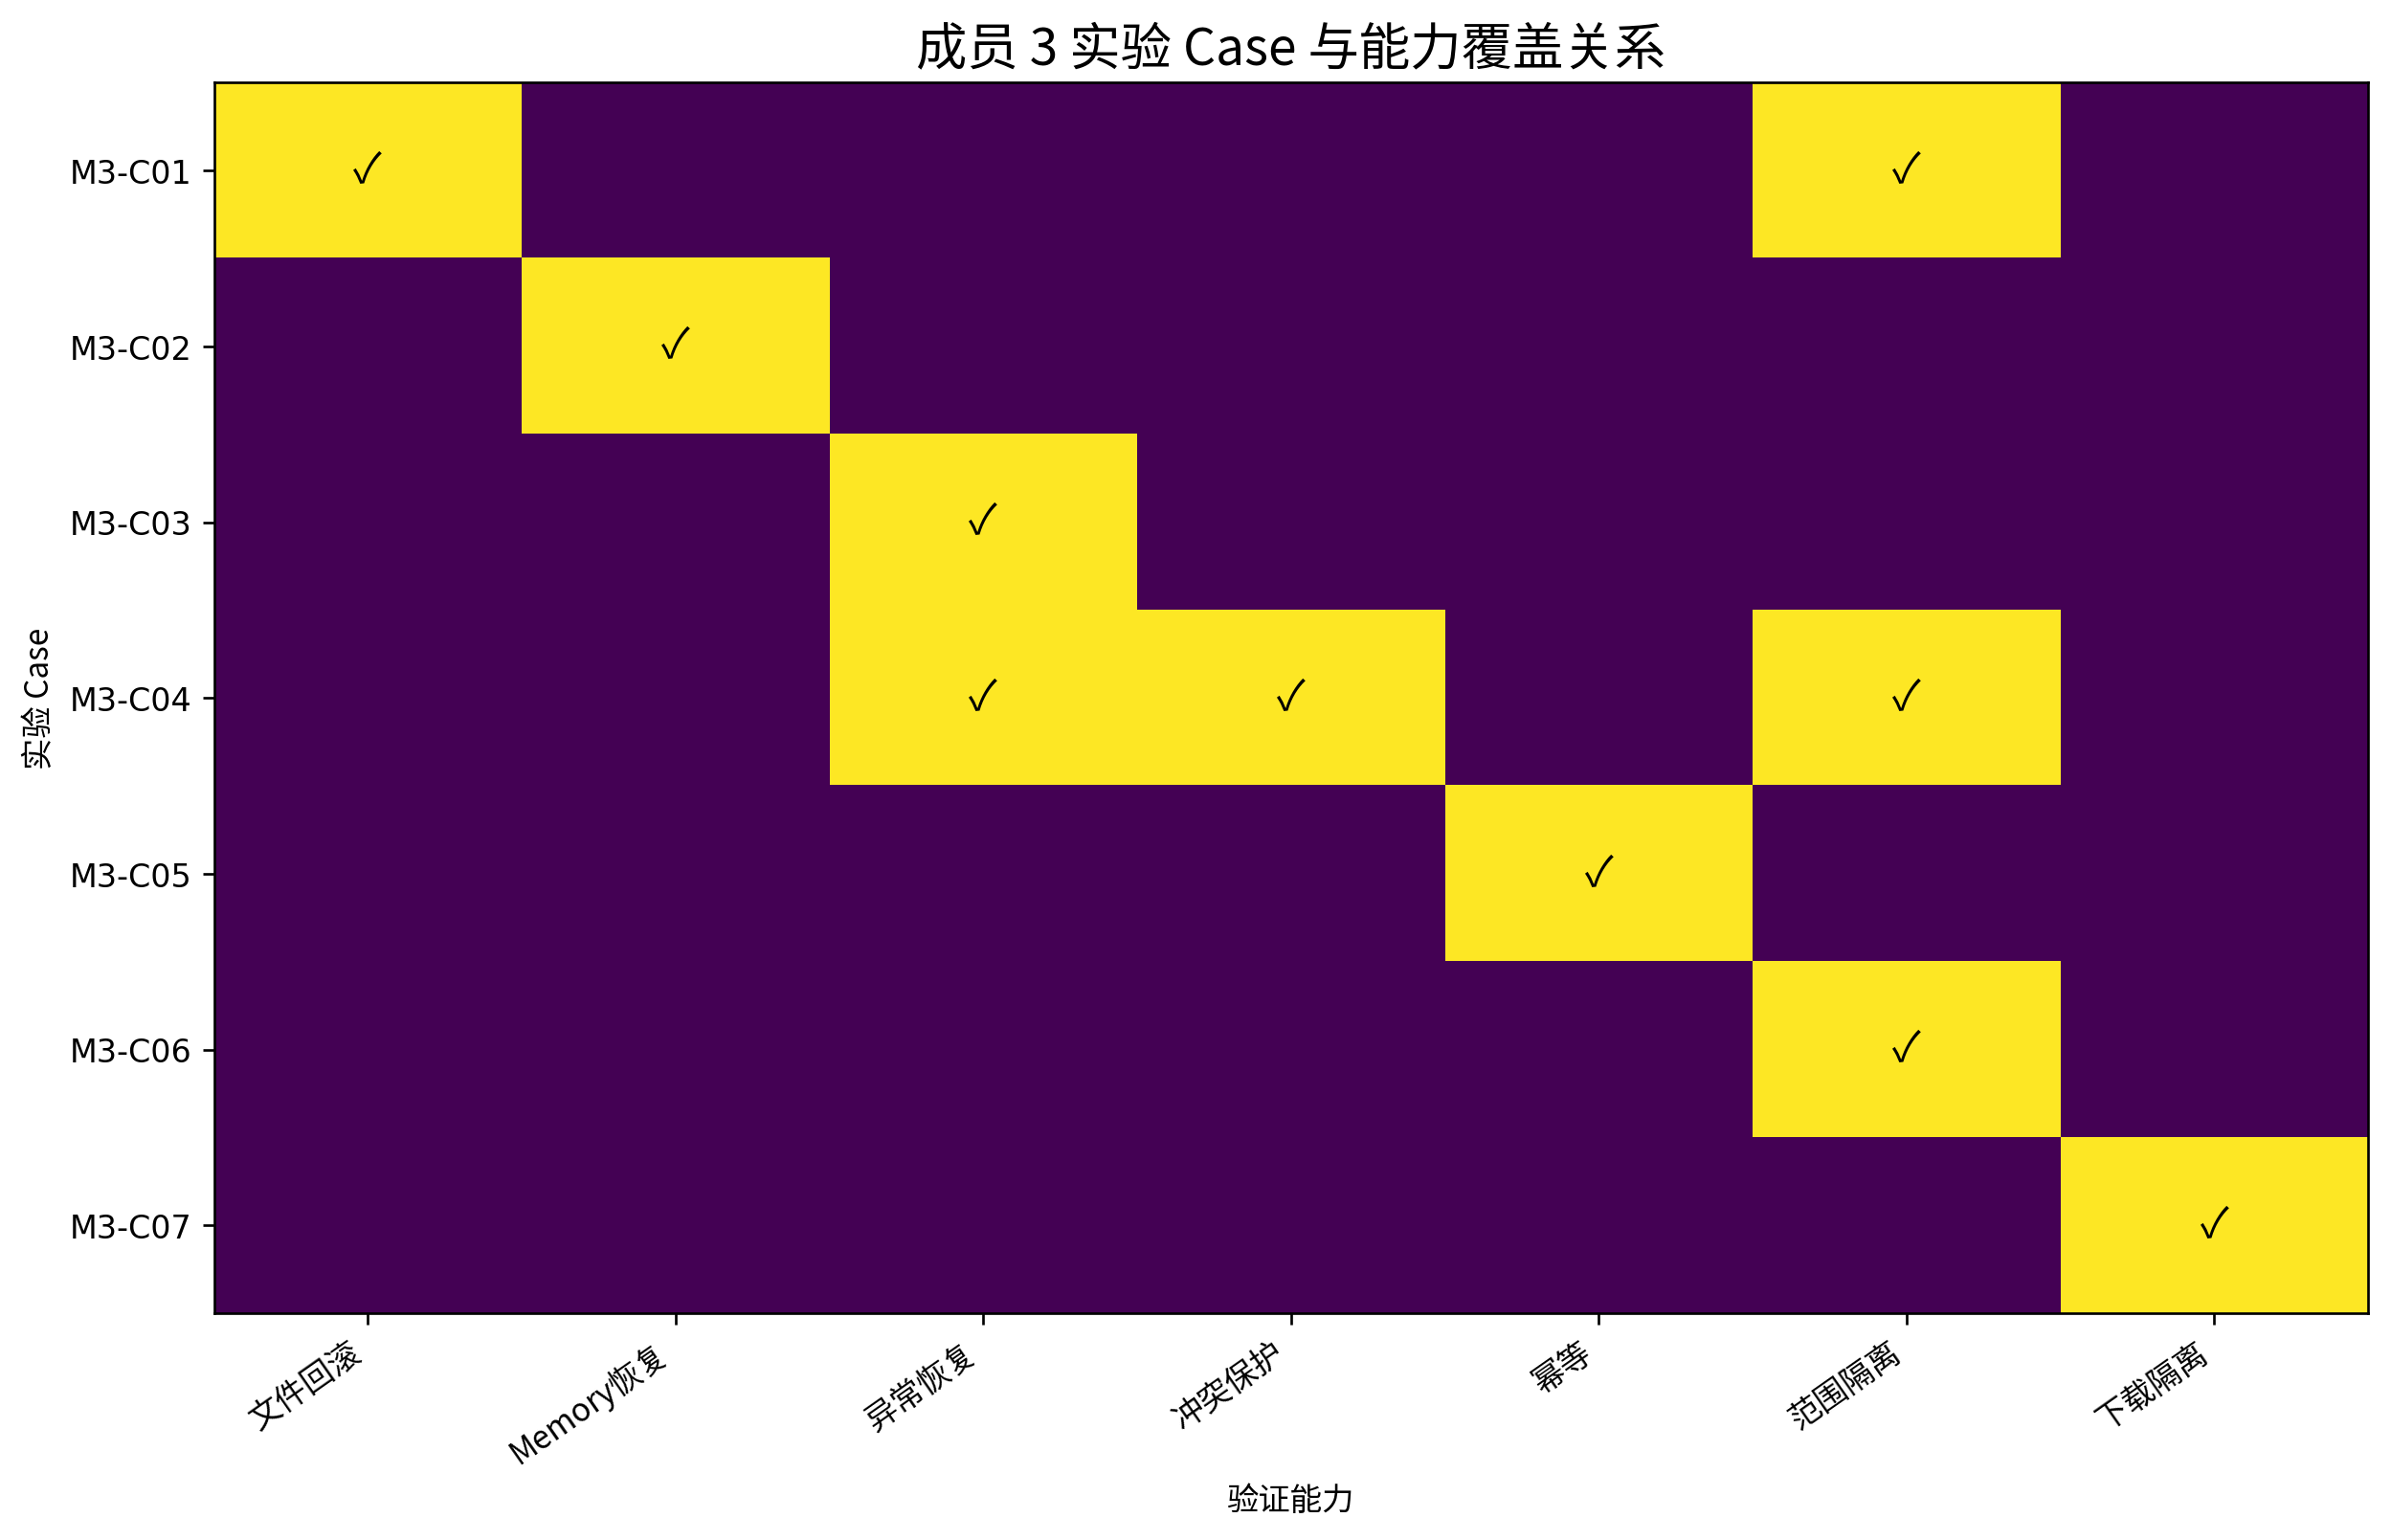
\includegraphics[width=0.90\linewidth]{member3_case_coverage.png}
  \caption{Rollback 正式实验的 Case 覆盖}
  \label{fig:rollback-coverage}
\end{figure}

图~\ref{fig:rollback-coverage} 展示七个 Case 与验证能力之间的对应关系。不同 Case 不是重复测试同一条路径，而是分别覆盖目标范围、Memory 状态、异常恢复、用户保护、重复执行、任务隔离和下载隔离等不同问题。这样安排的原因是，选择性回滚只有在这些条件同时成立时，才可以被理解为真正的“按影响范围恢复”。

表~\ref{tab:rollback-results} 给出三种模式的正式汇总结果。每种模式均包含 35 条记录。完整保护和自适应运行时模式的 Ground Truth 达标率为 100\%；自适应运行时模式的中位回滚耗时为 27 ms，平均保留 0.857 个独立 Effect。对照模式的达标率为 85.71\%，中位回滚耗时为 47 ms，平均保留 0.286 个独立 Effect。这里的结果不应被理解为不同模式的普适性能排名，而应结合实验设计理解：自适应模式依据显式范围处理受影响 Effect，因此在这些固定 Case 中减少了对无关成果的撤销。

\begin{table}[H]
  \centering
  \caption{Rollback 正式实验按 Mode 的汇总结果}
  \label{tab:rollback-results}
  \scriptsize
  \begin{tabular}{lrrrr}
    \toprule
    Mode & 记录数 & Ground Truth 达标率 & 中位回滚耗时/ms & 平均保留 Effect \\
    \midrule
    BASELINE & 35 & 85.71\% & 47 & 0.286 \\
    FULL\_GUARD & 35 & 100.00\% & 40 & 0.286 \\
    ADAPTIVE\_RUNTIME & 35 & 100.00\% & 27 & 0.857 \\
    \bottomrule
  \end{tabular}
\end{table}

图~\ref{fig:rollback-pass-rate} 进一步呈现三种模式的 Ground Truth 达标率。对照模式的未达标记录集中在提交元数据失败后的恢复情形；用户修改冲突产生的残留并不表示系统静默失败，而表示系统识别到用户已经写入新内容，选择不以旧状态覆盖新内容。跨任务范围拒绝在 Preflight 阶段完成，因而不会进入资源回滚。上述结果说明，回滚结果的好坏不能只看“是否把资源改回去”，还要看系统是否避免误删独立成果、是否尊重用户后写入内容、是否在范围越界时停止操作。

\begin{figure}[H]
  \centering
  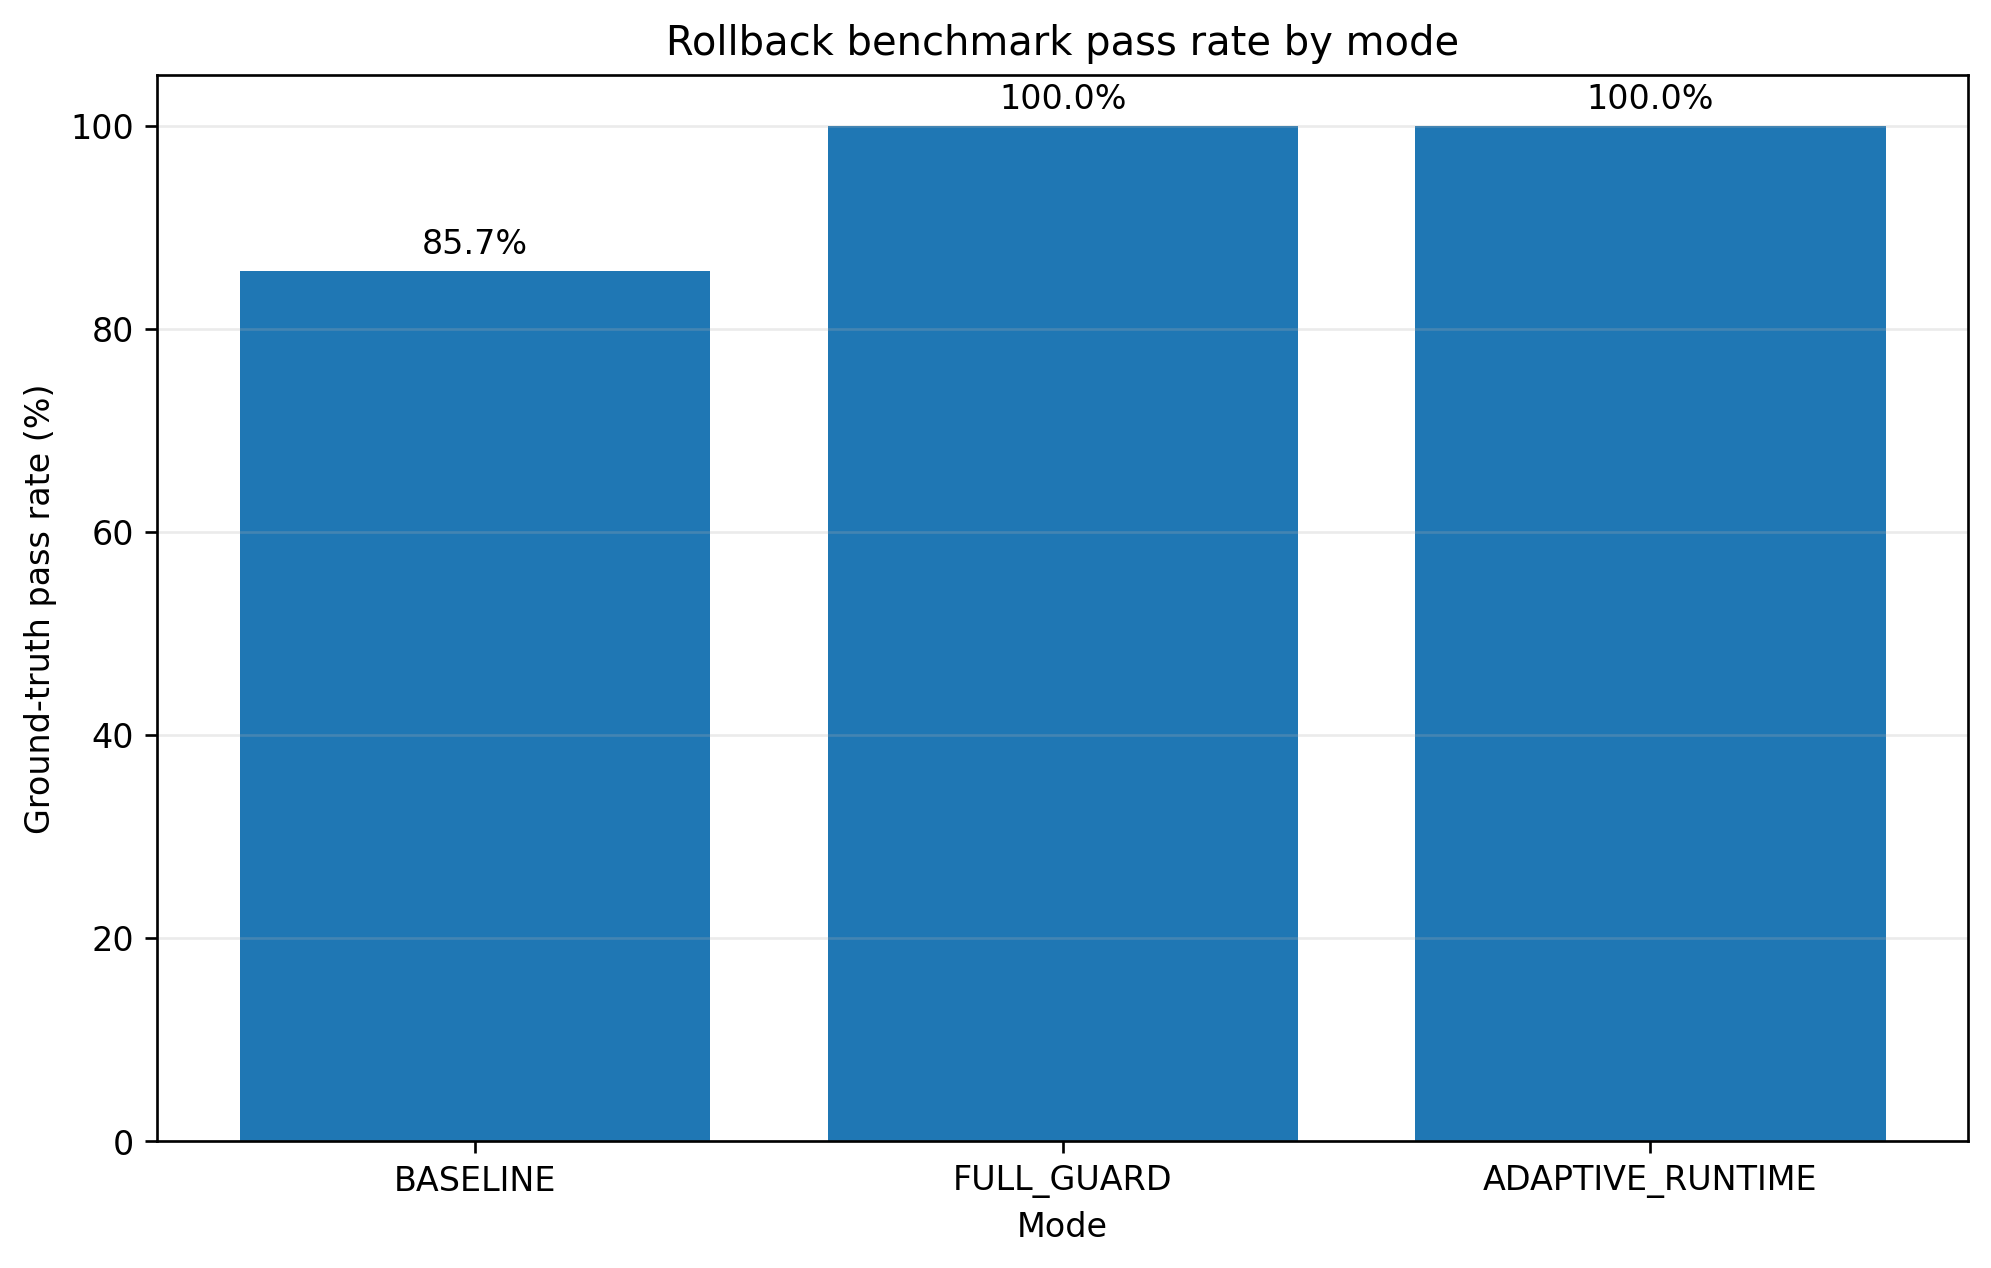
\includegraphics[width=0.82\linewidth]{rollback_success_rate_by_mode.png}
  \caption{Rollback 各 Mode 的 Ground Truth 达标率}
  \label{fig:rollback-pass-rate}
\end{figure}

Rollback 实验表明，Dependency-aware Selective Rollback 的价值不仅在于“能够回滚”，更在于“知道不该回滚什么”。在当前受控工程环境中，系统能够依据 Effect、Checkpoint、请求与任务关联处理受影响范围，并把独立成果的保留理由呈现为可追溯事实。它并不等同于对所有不可逆外部动作提供通用撤销能力，这一点也是作品始终保留的边界。

\section{浏览器场景与综合分析}

除三组正式实验外，作品还通过真实浏览器场景检查用户可见的闭环是否与运行时状态一致。场景包括：高风险节点进入等待审批后，用户 Grant 使图继续推进；用户 Deny 后目标及依赖路径被阻断；存在待处理 Effect 时用户 Cancel，受影响 Effect 回滚而独立 Effect 被保留；危险 Shell 输入被风险策略阻断并出现在 Audit 中。浏览器场景不使用静态前端结果，而是连接隔离的本地 Runtime，由真实的 EffectStore、Checkpoint 和 SelectiveRollbackExecutor 产生状态。

图~\ref{fig:browser-selective} 展示 Cancel 后的选择性回滚场景。界面中可以看到受影响的 Memory Effect 已变为 \code{ROLLED\_BACK}，独立的已提交 Effect 显示为 \code{PRESERVED}，并给出相应的安全生命周期原因。该场景把第二章中的机制说明转化为用户能够直接观察的结果：取消并不意味着无差别删除，而是以实际影响范围为依据处理状态。

\begin{figure}[H]
  \centering
  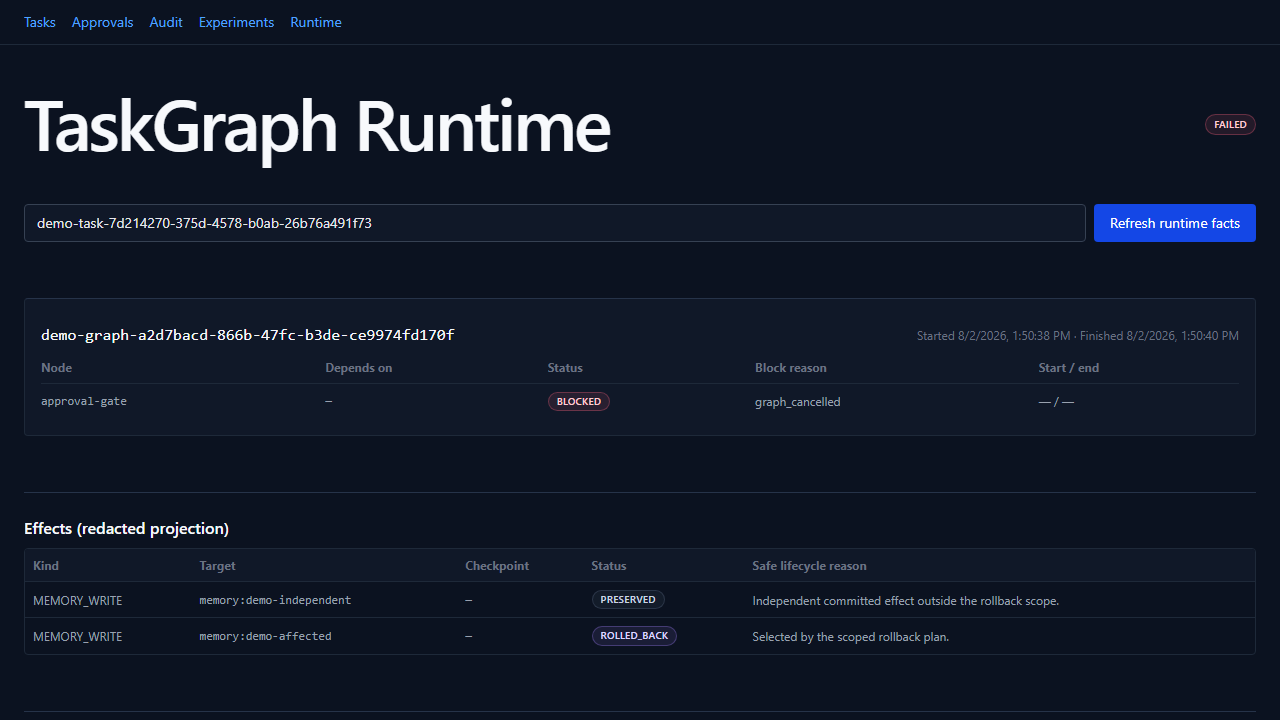
\includegraphics[width=0.96\linewidth]{selective-rollback-preserved.png}
  \caption{本地浏览器场景：Cancel 后的回滚与独立 Effect 保留}
  \label{fig:browser-selective}
\end{figure}

图~\ref{fig:browser-security} 展示危险 Shell 输入被阻断并写入 Audit 时间线的场景。页面仅呈现任务状态、事件类型和安全理由等脱敏信息，不显示密钥、原始不可信内容或隐藏推理。结合安全、调度和回滚实验可以看到，作品的三个核心机制并不是彼此孤立的：风险策略决定动作能否进入下一阶段，审批状态影响任务图推进，Effect 与 Checkpoint 决定取消后如何处理资源，Audit 则把整个过程连接为可回溯的记录。

\begin{figure}[H]
  \centering
  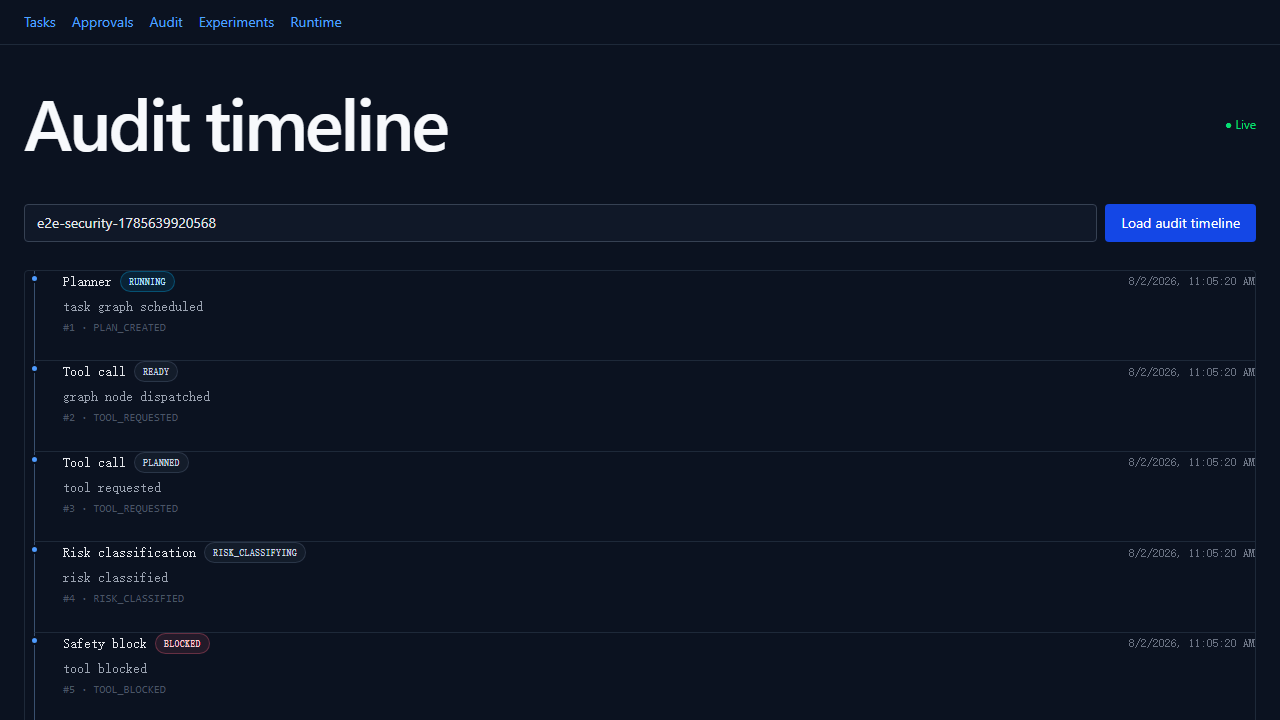
\includegraphics[width=0.96\linewidth]{security-blocked-audit.png}
  \caption{本地浏览器场景：危险 Shell 阻断与 Audit 记录}
  \label{fig:browser-security}
\end{figure}

三组正式实验与浏览器场景共同说明：Aegis Runtime 的安全性不只体现在某个页面的提示信息上，而体现在一次任务从风险判断、审批等待、节点推进、Effect 提交到取消回滚的连续行为中。系统最终验收通过；其结论范围限定在本作品使用的固定场景和受控运行环境内。

\chapter{创新性说明}

\section{Transactional Controlled Execution}

第一项核心创新是 \textbf{Transactional Controlled Execution}。它将可恢复副作用置于可检查的 Effect 生命周期中，以 Checkpoint、Pending、验证、Commit、Rollback 和 Cleanup 约束真实资源何时可见、何时可信和何时可恢复。该机制把工具调用从“函数返回即完成”改为具有关联关系和状态边界的受控执行过程，但不宣称完整 ACID、分布式事务或服务重启恢复。

\section{Approval-aware TaskGraph Scheduling}

第二项核心创新是 \textbf{Approval-aware TaskGraph Scheduling}。它把审批状态与任务依赖和 Effect target 冲突范围一同纳入调度决策：等待审批的节点不会越过安全边界，其后继或冲突节点受到约束，而无依赖、无冲突的独立节点可以继续推进。Grant、Deny 与 Cancel 分别导致可验证的恢复、阻断和收敛状态；同一节点 speculative overlap 明确为 \code{NOT\_SUPPORTED}。

\section{Dependency-aware Selective Rollback}

第三项核心创新是 \textbf{Dependency-aware Selective Rollback}。它以 TaskGraph、Effect、request 和 Checkpoint 的关联关系定位受影响依赖闭包：回滚处于该范围内的可恢复 Effect，保留范围外且已安全提交的独立 Effect，并通过脱敏状态与 Audit 记录解释回滚或保留原因。该机制区别于按整任务清空的粗粒度恢复，也不将不可逆外部行为宣称为本地可撤销资源。

\section{支撑机制与组合边界}

Risk、Policy、Permission、Approval 与 Audit 不是独立的核心创新命名，而是使三项机制可执行、可验证和可追溯的支撑层。它们对不可信提案采用 Fail-Closed 的运行时边界，绑定审批对象与实际执行请求，并以结构化事实连接节点、Effect 和资源状态。作品的创新落点是上述三项机制在同一 Runtime 内的组合与工程闭环，而不是声称单独发明风险评估、人工审批或审计本身。

\chapter{总结}

\section{工作总结}

本作品围绕“如何让 Agent 的真实行动处于可控状态”这一问题，设计并实现了 Aegis Runtime。系统不把安全理解为模型在生成文本时的一次自我判断，而是把风险判断、策略与权限、人工审批、任务图调度、Effect 生命周期、提交与回滚、Audit 记录放入连续的运行时过程。用户提交的任务因此不再只是一个黑盒执行过程：系统能够说明某个节点为何等待、某项资源是否已经提交、取消后哪些影响被恢复、哪些独立成果被保留。

作品以 Transactional Controlled Execution、Approval-aware TaskGraph Scheduling 和 Dependency-aware Selective Rollback 为三项核心创新。第一项机制使可恢复副作用具有 Pending、校验、提交或回滚的明确边界，避免将候选结果过早视为可信成果；第二项机制让审批状态参与任务图调度，使等待审批的节点及其受影响范围得到约束，同时允许安全独立节点继续推进；第三项机制依据任务、请求、Effect、Checkpoint 和资源目标之间的关联进行局部恢复，避免因为一个问题误删全部独立成果。

三组正式实验分别检验安全处置、图调度和状态恢复，浏览器场景进一步呈现 Grant、Deny、Cancel、危险操作阻断和 Audit 记录等用户可见闭环。实验和场景共同说明，作品的价值不只在于“检测到风险”，而在于风险判断能够改变真实执行路径；不只在于“支持审批”，而在于审批决定能够影响图的推进；不只在于“可以回滚”，而在于回滚能够按影响范围处理并保护独立成果。系统最终验收通过。

\section{作品意义}

对使用者而言，Aegis Runtime 将复杂的 Agent 执行过程转化为可以理解的状态：等待审批不再是模糊的停顿，提交不再只是没有依据的成功提示，取消也不再意味着不确定的后台行为。用户能够在任务、审批、Effect 和 Audit 视图之间追踪同一事项，并据此作出授权、拒绝或取消决定。脱敏展示使这种可见性不以暴露密钥、原始不可信内容或隐藏推理为代价。

对开发者而言，统一的关联关系为系统测试和问题排查提供了基础。风险判断、审批事件、图节点、Effect 和资源处理不再各自留下难以对应的日志，而是围绕 task、request 和 Checkpoint 等事实建立联系。这样，当出现异常时，可以检查问题发生在风险判定、审批处理、调度推进还是资源恢复阶段；当需要增加新的可恢复工具时，也可以沿用既有的受控执行与 Effect 记录方式。

从更广泛的 Agent 安全实践看，本作品说明运行时治理需要同时考虑预防、约束和恢复。只做输入过滤无法覆盖工具调用之后的状态变化，只做人工审批无法保证审批决定与任务调度一致，只做异常捕获也无法决定哪些成果应被保留。将三类问题放在同一条可追溯链路中，能够使安全机制从单点规则进一步发展为可验证的系统行为。

\section{局限性}

本系统是单进程、受控环境中的 Runtime 原型。当前原型未覆盖分布式工作流编排、服务重启恢复、完整 ACID 语义、通用 MCP/Skill 协议和同一节点 speculative execution。选择性回滚仅适用于已经纳入 Effect、Checkpoint 和关联关系管理的可恢复状态；对于真实支付、邮件发送或其他不可逆外部动作，系统不能宣称具有通用的事后撤销能力，只能在动作释放前通过审批、策略和提交边界降低风险。

实验采用固定 fixtures、确定性规则和受控时延，重点验证机制行为、状态一致性和结果可复核性。Safety 正式结论不依赖 LLM 裁决，Graph 实验也不用于说明统计显著性或真实大模型在开放环境中的性能。开放网络中的输入变化、第三方服务差异、长时间运行与多进程协调都会带来额外挑战，因此本作品的结论应理解为对当前工程范围内机制的验证，而不是对所有 Agent 应用场景的普适保证。

\section{未来工作}

后续工作可以在不改变安全边界的前提下，逐步扩展状态协调能力。例如，可研究 TaskGraph、审批与 Effect 状态在受控持久化条件下的恢复方式，并明确恢复过程中应当重新核验的授权和资源条件；对于数据库写入、网络请求和第三方 API，可进一步区分可逆、可补偿和不可逆操作，并为不同类别设计更明确的提交条件与用户确认方式。

在交互层面，未来可以继续优化风险理由、审批摘要和 Audit 查询，使不同技术背景的用户更容易理解系统为何提出确认、为何阻断某个动作以及为何保留某项独立成果。在实验层面，可在保持可复核和不夸大结论的前提下，增加更多类型的受控业务流程，并考察不同资源冲突与长期任务场景下的状态一致性。无论功能如何扩展，核心原则仍应保持：任何新增执行能力都需要先说明其授权边界、可观察状态和异常后的处理方式。


\printbibliography[title={参考文献}]

\end{document}
